\glsresetall
\chapter{Results, Analysis and Limitations}
\label{chap:results_analysis_and_limitations}

In this Chapter we present the results gathered from the ``Data Analysis'' component presented in Chapter~\ref{chap:proposed_solution}~-~\nameref{chap:proposed_solution}, to answer the questions defined in Section~\ref{sec:research_questions}. Results for both questions, ``1. Is there any anomalous service?'' and ``2. How can we measure the quality of tracing?'', are presented as well as a brief discussion regarding both results.

\section{Anomaly Detection}
\label{sec:anomaly_detection}

For the first question, the approach was use the OTP tool to extract metrics from tracing data to further analyse it using the unsupervised learning algorithm. The implemented algorithm used for metrics extraction is presented in Algorithm~\ref{alg:metrics_extraction_from_tracing}.

After extract metrics, a tool for metrics visualisation (e.g., Grafana) can be used to visualise the metrics from the Time-Series database.

\todo{Explain path until arrive at data in Figure~\ref{fig:comparison_anomalous_non_anomalous_regions} -- ADD FIGURE with anomalies.}

Figure~\ref{fig:comparison_anomalous_non_anomalous_regions} provides a representation of two time-frame samples, one for the ``anomalous'' region, and the other for the ``non-anomalous'' region considering the same service. In this samples we retrieved data to analyse and give answers to the first question. We considered three features (as shown in the samples bellow): the number of incoming requests, the number of outgoing requests and the average response time. The sample resolution for the time-frame is 10 minutes.

\begin{figure}
  \centering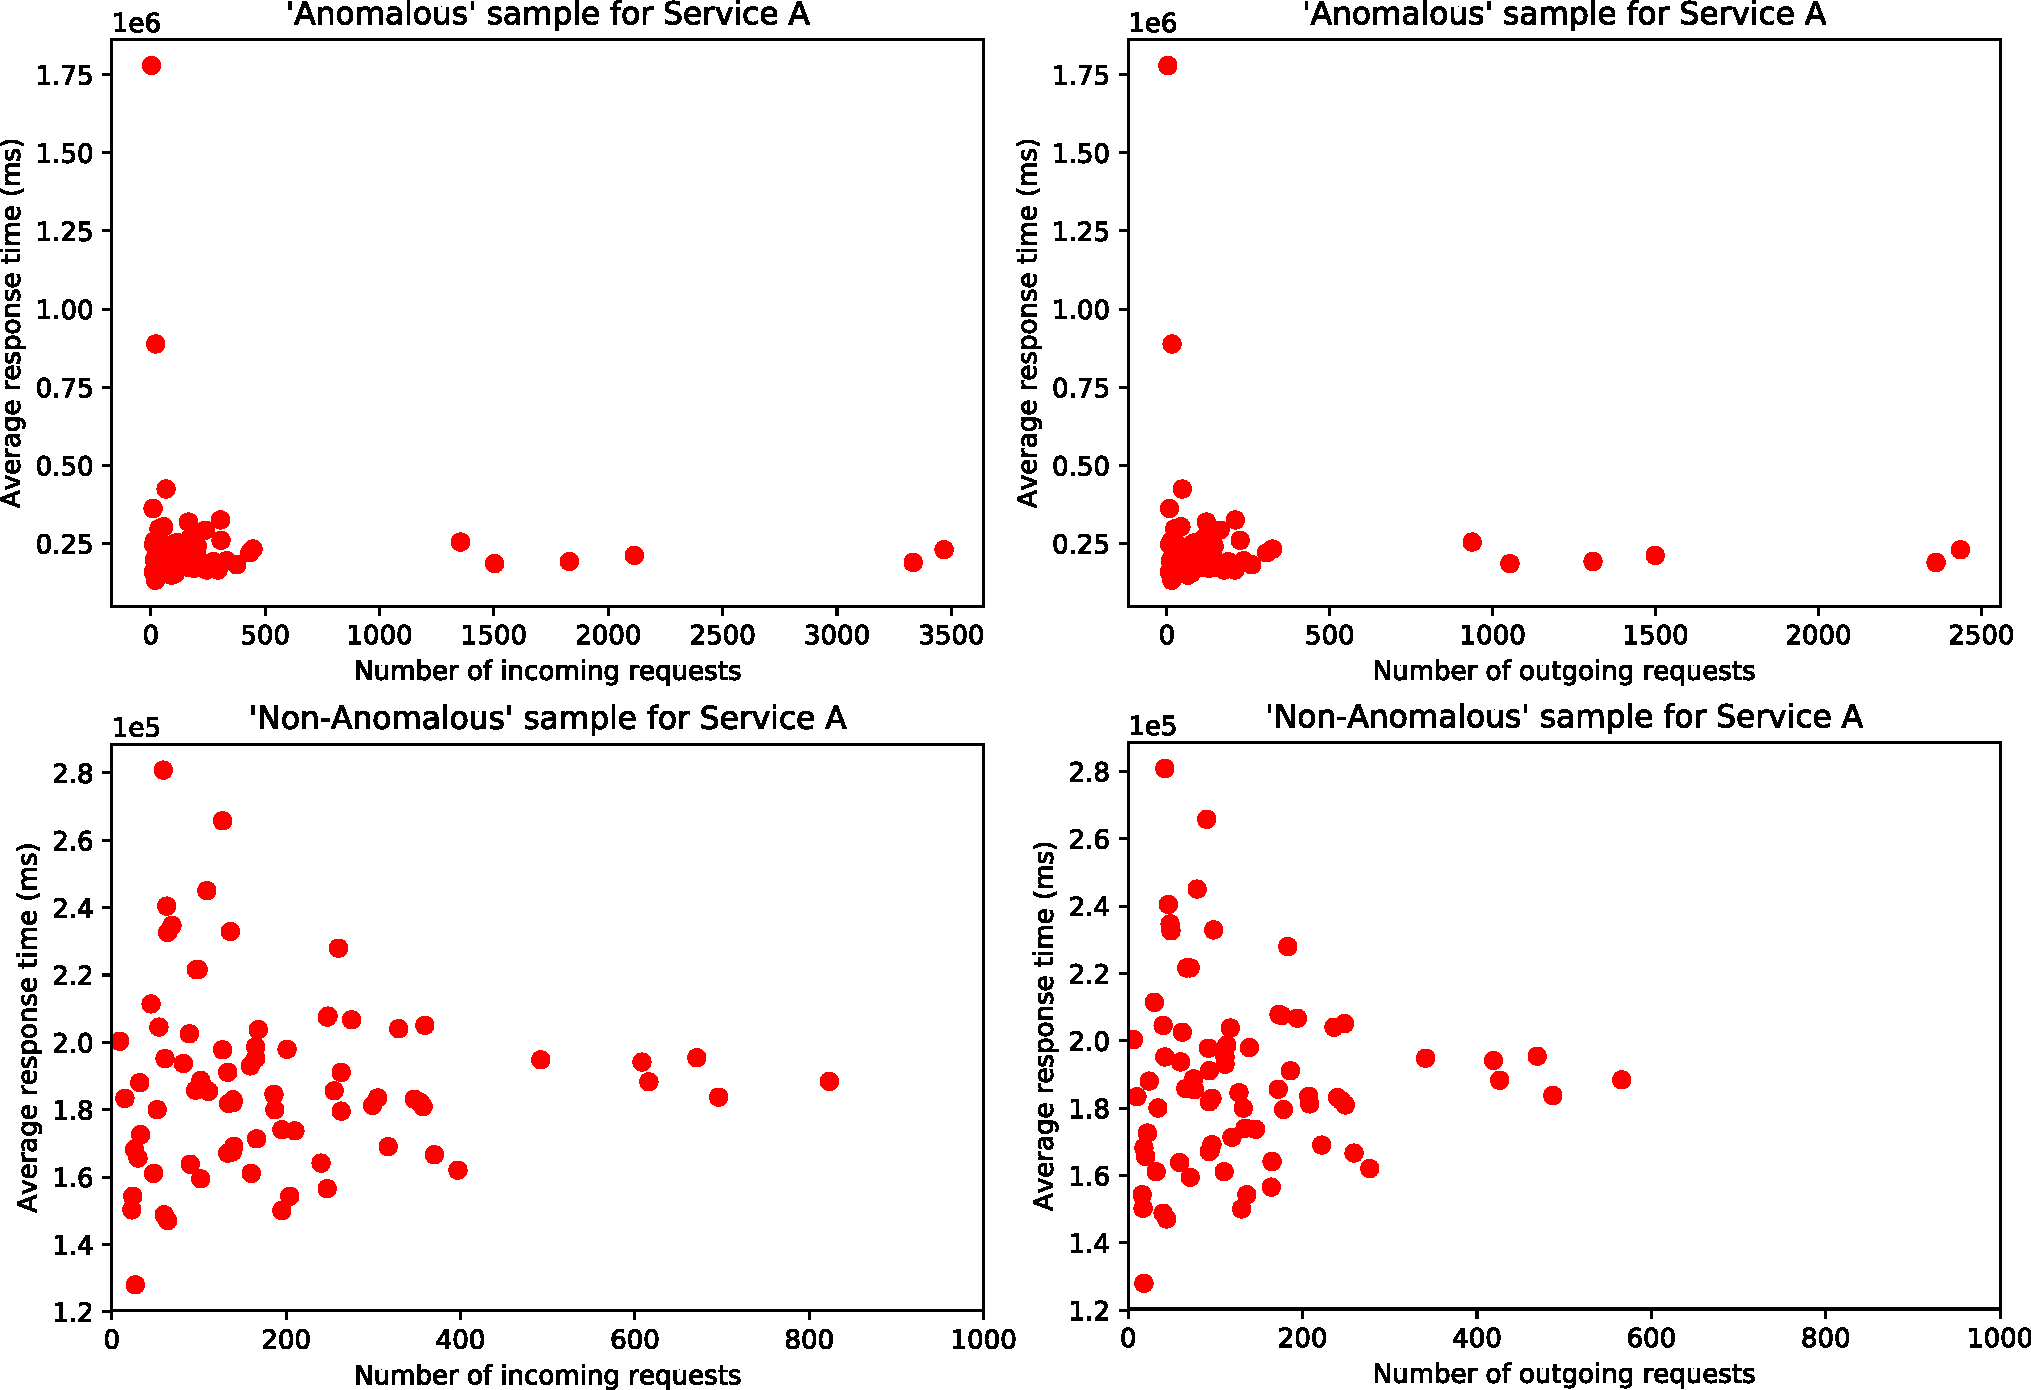
\includegraphics[width=1.0\linewidth]{images/result_samples_for_service_a.pdf}
  \caption{Comparison between ``Anomalous'' and ``Non-Anomalous'' service time-frame regions.}
  \label{fig:comparison_anomalous_non_anomalous_regions}
\end{figure}

As we can see in Figure~\ref{fig:comparison_anomalous_non_anomalous_regions}, there is a clear difference between anomalous and non-anomalous regions. There is a drastic change in the range of values between the anomalous and non-anomalous regions, where the maximum for each feature changes drastically and therefore, outliers are visible and evident in the observations. In the anomalous samples, it is possible to notice a clear crowding of points near the origin point of the chart and some outliers in the upper-left and down-right regions of the chart. On the other side, in the non-anomalous samples, all that is possible to notice is the crowding of points near the origin point of the chart. The crowding of points is what is expected to be the normal behaviour for services, which means that is expected that the service can handle the load with good response times. Furthermore, after this observations, what is expected is to investigate what these points represent and what is causing this unexpected increment in the number of incoming/outgoing requests and the average response time. There are two anomalous situations observed:

\begin{enumerate}
  \item Services are increasing the response time when there are few incoming/outgoing requests.
  \item Services are receiving more incoming/outgoing requests, however it is having a good response time.
\end{enumerate}

The first situation is much worse than the second one. The expectation is that services can handle more requests and keep the average response time. The worst case scenario would be to find points in the upper-right section of the charts, however this was not observed in this tracing data.

After this, and to study both situations, an analysis of trace request work-flow types was performed. The objective of this analysis is to perceive if there is some strange occurrences in request work-flow paths. To be able to do this, the OTP must be able to get the tracing data and map each unique trace work-flow for the given time-frame. The algorithm is presented in Algorithm~\ref{alg:work_flow_type_algorithm}:

\todo{Mentioned in Section 6.1}
\begin{algorithm}
  \KwData{Trace files/Trace data.}
  \KwResult{\gls{csv} with unique workflow types, their corresponding count and times.}
  Read start\_time and end\_time from configuration\;
  Read SpanList from trace files/trace data within defined time\_frame\;
  \While{have Spans in SpanList}{
    Read Span\;
    Map Span to SpanTrees\;
    Read SpanTree\;
    Map SpanTree to TraceInfos\;
    Read TraceInfo\;
    Read workflows, workflow count, times, (others) from TraceInfo\;
    Write fields to \gls{csv} files\;
  }
  \caption{Work-flow type algorithm.}
  \label{alg:work_flow_type_algorithm_2}
\end{algorithm}

As presented in algorithm~\ref{alg:work_flow_type_algorithm}, parameters from TraceInfo are written to the \gls{csv} files. These files are then processed in the ``Data Analyser'' component. Interesting results, from ``Anomalous'' and ``Non-Anomalous'' regions of the services work-flow types are presented in Figure~\ref{fig:work_flow_type_analysis}.

\begin{figure}
  \centerline{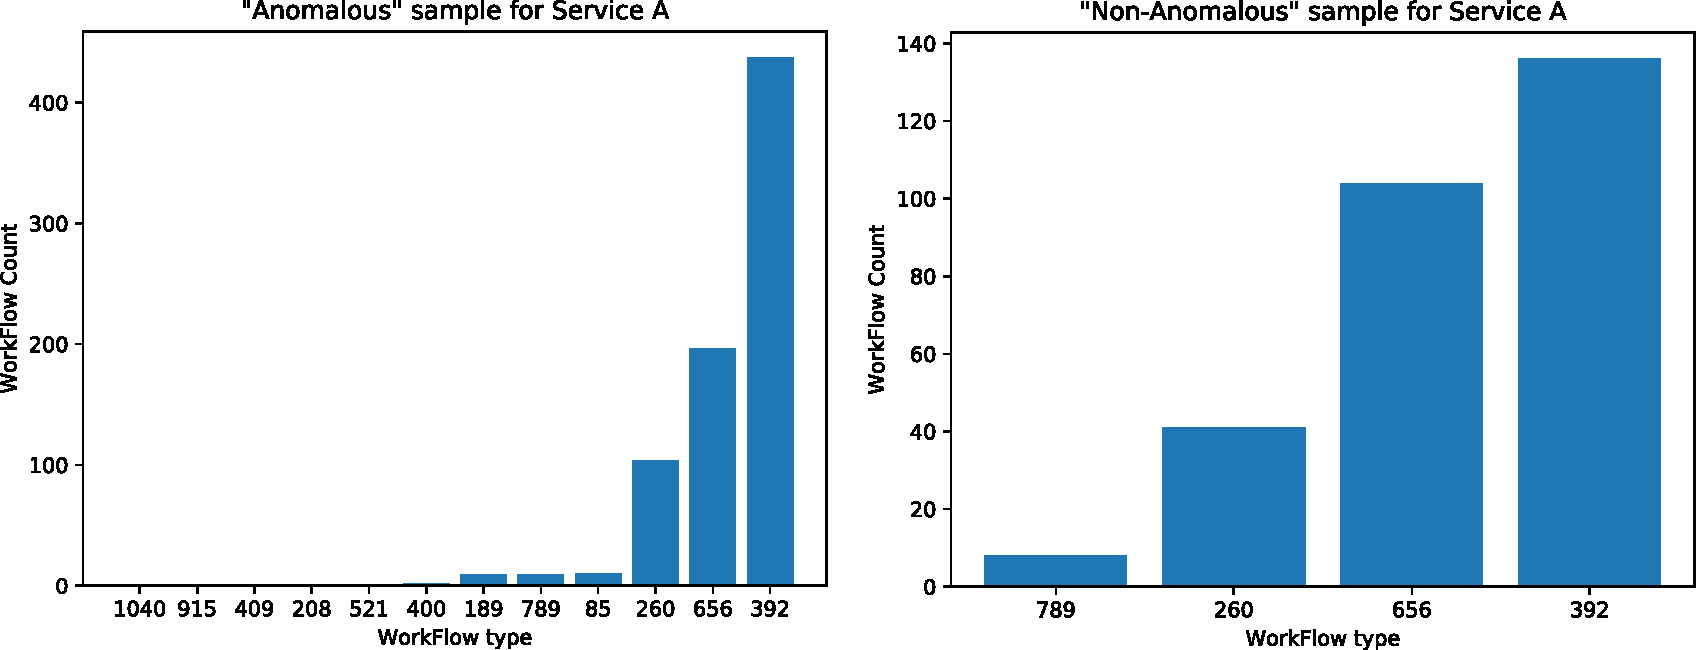
\includegraphics[width=1.0\linewidth]{images/workflow_type_count.pdf}}
  \caption{Comparison between ``Anomalous'' and ``Non-Anomalous'' service work-flow types.}
  \label{fig:work_flow_type_analysis}
\end{figure}

One interesting thing to notice and that proves this method is that, in the anomalous regions, more quantity and more types of request work-flow types were observed. The next step was to check what was causing this by retrieving the most ``called'' work-flow, however the results were not good because of the completeness of the tracing data. The flows were not relevant for a further analysis because they were just calls from point A to B. At this point, and for this question, it is possible to say that this data set was exhaustively analysed, and an improvement of the tracing data should be a path to take. One point to note for future work is to test this method with other tracing data to understand the root cause of the anomalous behaviour.

\section{Trace Quality Analysis}
\label{sec:trace_quality_analysis}

For the second question, the approach was the same as in the previous question, use the OTP to process the tracing data and gather the results to be further analysed in the ``Data Analysis'' component. However, in this case, the results obtained by the first component were directly used by the second component.

In this question the analysis is divided in two procedures as explained in Chapter~\ref{chap:proposed_solution}.

The first procedure aims to check if the spans comply with the OpenTracing specification. The method is rather simple and is presented in Algorithm~\ref{alg:span_structure_analysis_algorithm}.

\todo{Mentioned in Section 6.1}
\begin{algorithm}
  \KwData{Trace files/Trace data.}
  \KwResult{\gls{csv} file reporting span structure analysis.}
  Read specification from open\_tracing\_specification\_schema.json\;
  \While{not end of tracing}{
    Read Span\;
    Check Span against specification\;
  }
  Write results from ``Check'' to \gls{csv} file\;
  \caption{Span structure analysis algorithm.}
  \label{alg:span_structure_analysis_algorithm_2}
\end{algorithm}

The results obtained by this method were that every span structure complies with the specification. This is not a very good test because the specification of the OpenTracing is not very strict and therefore, the created method for testing does not provide a very accurate kind of results. For example, the units for timestamps are not uniform, one can use milliseconds and in other field of a span presented in the same trace, other can use microseconds. This leads to problems in time measurements and is not covered by this test. The redefinition of the specification is discussed in Chapter~\ref{chap:conclusion_and_future_work}.

\todo{Check bellow because it was explained in Ch.6.}

The second procedure aims to check if tracing covers the entire time of the root spans. For a simple example, if we have a trace with a root span of 100 milliseconds of duration, and this root span has two children spans, one with $50ms$, the other one with $10ms$, the entire trace has a coverage of $(50+10)/100=60\%$. This method is applied to every trace, and the results are plotted for visualisation. In this case we apply it and split the results by service, with the objective of perceive the time coverability of tracing in each service. The method is presented in Algorithm~\ref{alg:trace_coverability_analysis} and the corresponding results, regarding two different services, are presented in Figure~\ref{fig:services_coverability_analysis}.

\todo{Mentioned in Section 6.1}
\begin{algorithm}
  \KwData{Trace files/Trace data.}
  \KwResult{\gls{csv} file for each service reporting the coverability analysis.}
  Read start\_time and end\_time from configuration\;
  Get services from Zipkin\;
  \While{service in services}{
    Get traces from Zipkin using service, start\_time and end\_time\;
    Map traces in SpanTrees\;
    Calculate trace\_coverability using SpanTrees\;
    Write trace\_coverability to \gls{csv} file\;
  }
  \caption{Trace coverability analysis algorithm.}
  \label{alg:trace_coverability_analysis_2}
\end{algorithm}

\begin{figure}
  \centering{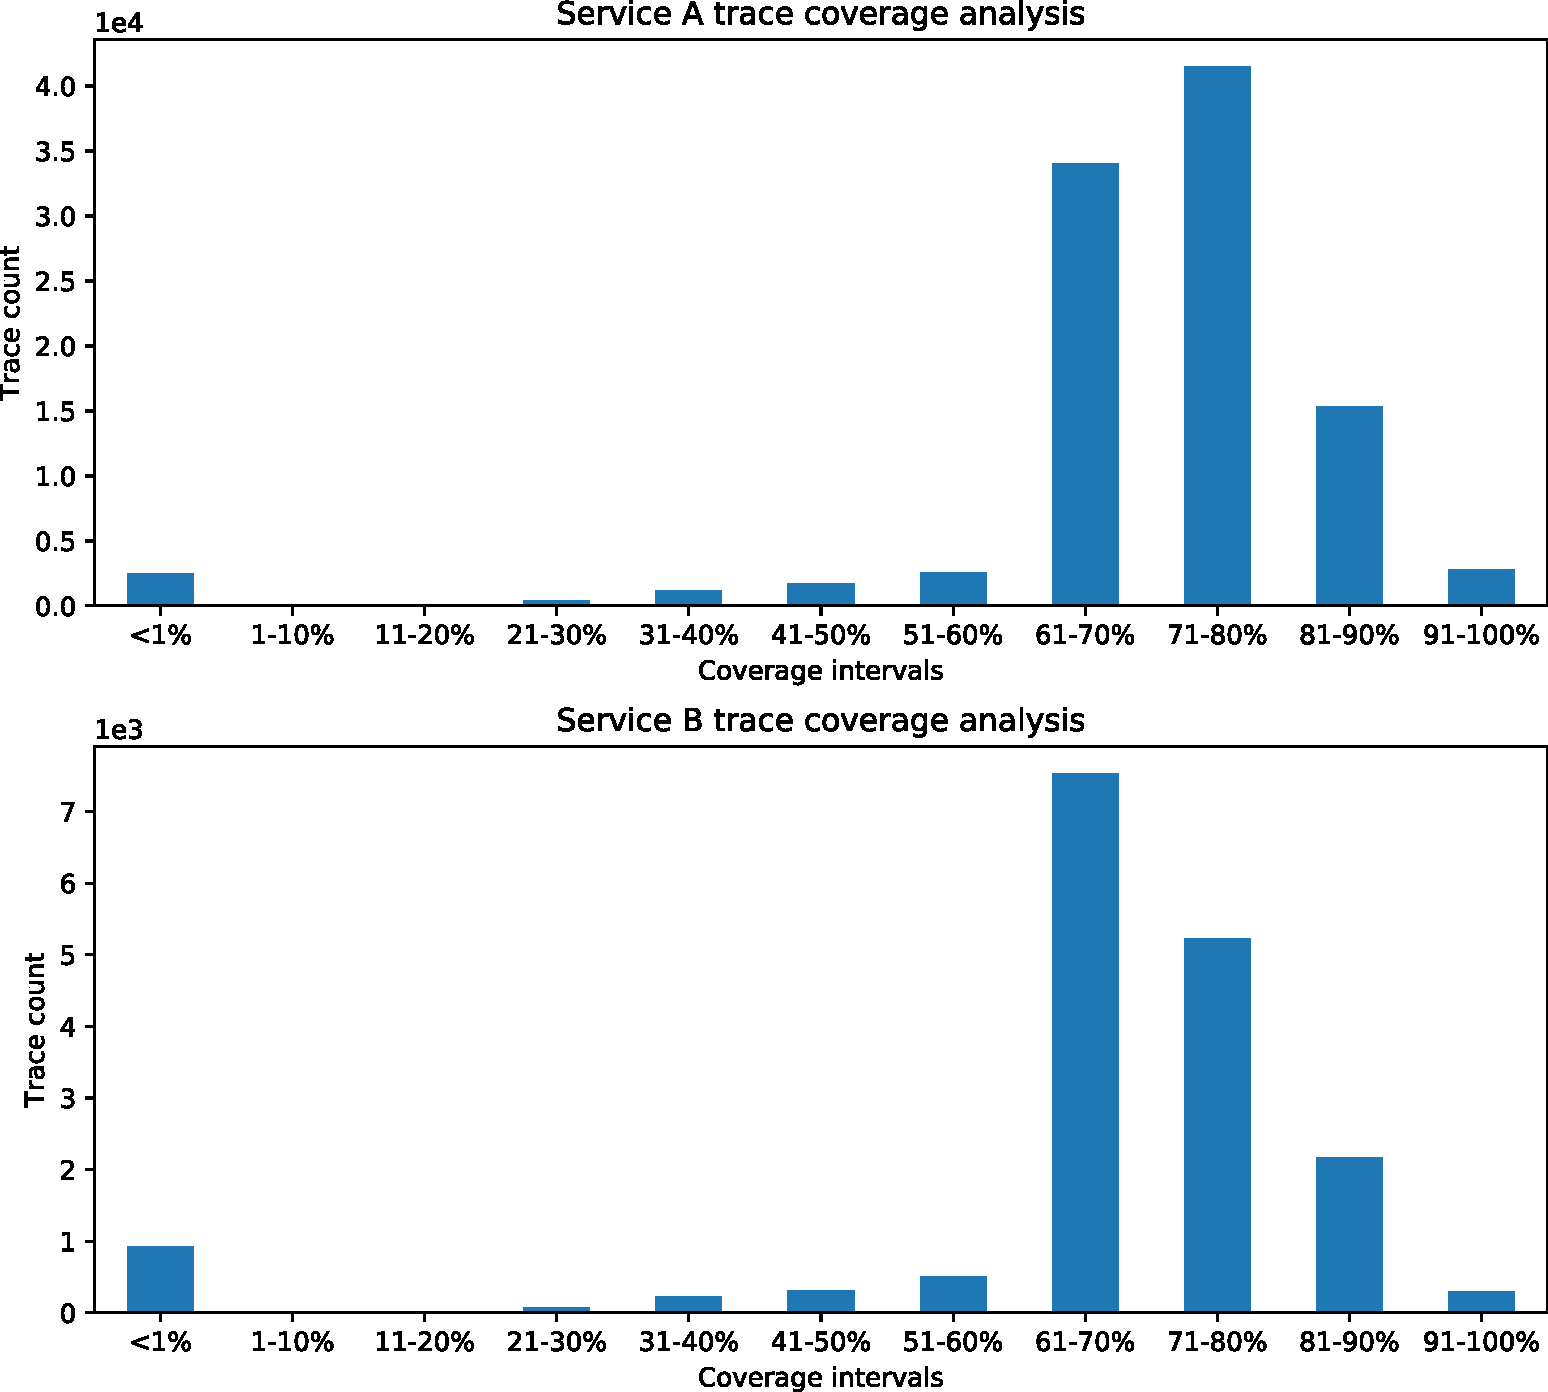
\includegraphics[width=1.0\linewidth]{images/service_trace_coverability_analysis.pdf}}
  \caption{Services coverability analysis.}
  \label{fig:services_coverability_analysis}
\end{figure}

Figure~\ref{fig:services_coverability_analysis} allows the user to visualise the tracing coverability, in terms of how many the overall tracing covers their entire execution duration. The most important thing to notice is the presence of higher bar values in $60\%-100\%$ regions. This means that coverability for this tracing could be better, but in overall is good. What is expected by the result of this kind of analysis is that the coverability of tracing remains closer to the last interval $(90\%-100\%)$, which means that our service is fully/almost fully covered by this kind of data and therefore, the analysis of this data is worthy and the results provided by the usage of this data are trusty. From this data set, the results for each service where close to what is shown by this figure. From this analysis, one thing to improve is to develop a method to analyse the gathered results in order to detect traces that do not cover their duration with respect to a predefined threshold. This would allow developers to improve their tracing coverage.

\section{Limitations of OpenTracing Data}
\label{sec:limitations_of_opentracing_data}

\todo{...}

\checkoddpage
\ifthenelse{\boolean{oddpage}}
{ % Odd page
\newpage
\blankpage}
{ % Even page
}